\documentclass[11pt,a4paper]{article}

% ============ PACKAGES ============
\usepackage[utf8]{inputenc}
\usepackage[T1]{fontenc}
\usepackage[margin=1in]{geometry}
\sloppy
\usepackage{amsmath,amssymb,amsthm}
\usepackage{booktabs}
\usepackage{array}
\usepackage{enumitem}
\usepackage{fancyhdr}
\usepackage{hyperref}
\usepackage{xcolor}
\usepackage{tcolorbox}
\tcbuselibrary{breakable}
\usepackage{float}
\usepackage{listings}
\usepackage{tikz}
\usetikzlibrary{shapes.geometric, arrows.meta, positioning, fit}

% ============ COLORS ============
\definecolor{codeblue}{rgb}{0.13,0.29,0.53}
\definecolor{passgreen}{rgb}{0,0.5,0}
\definecolor{failred}{rgb}{0.8,0,0}
\definecolor{codegray}{rgb}{0.5,0.5,0.5}
\definecolor{backcolour}{rgb}{0.97,0.97,0.97}
\definecolor{notebg}{rgb}{0.93,0.95,1.0}
\definecolor{noteborder}{rgb}{0.4,0.5,0.7}
\definecolor{warningbg}{rgb}{1.0,0.97,0.88}
\definecolor{warningborder}{rgb}{1.0,0.6,0.0}
\definecolor{scenariobg}{rgb}{0.95,1.0,0.95}
\definecolor{scenarioborder}{rgb}{0.2,0.6,0.3}

% ============ THEOREM ENVIRONMENTS ============
\theoremstyle{definition}
\newtheorem{definition}{Definition}[section]
\newtheorem{invariant}{Invariant}[section]

% ============ BOXES ============
\newtcolorbox{notebox}{
    colback=notebg, colframe=noteborder, boxrule=1pt,
    left=6pt, right=6pt, top=6pt, bottom=6pt
}

\newtcolorbox{warningbox}[1][Volume Dependency]{
    colback=warningbg, colframe=warningborder, boxrule=1.5pt,
    left=6pt, right=6pt, top=6pt, bottom=6pt,
    fonttitle=\bfseries, title={#1}
}

\newtcolorbox{scenariobox}[1][Worked Scenario]{
    colback=scenariobg, colframe=scenarioborder, boxrule=1.5pt,
    left=8pt, right=8pt, top=8pt, bottom=8pt,
    fonttitle=\bfseries, title={#1}, breakable
}

% ============ CODE STYLE ============
\lstdefinestyle{pythonstyle}{
    backgroundcolor=\color{backcolour},
    basicstyle=\ttfamily\footnotesize,
    keywordstyle=\color{codeblue}\bfseries,
    commentstyle=\color{passgreen},
    breaklines=true, frame=single, numbers=left, numbersep=5pt
}
\lstset{style=pythonstyle}

% ============ HEADERS ============
\pagestyle{fancy}
\fancyhf{}
\fancyhead[L]{\textit{EFM Codex --- Appendix C}}
\fancyhead[R]{\thepage}

% ============ HYPERREF ============
\hypersetup{
    colorlinks=true, linkcolor=codeblue, urlcolor=cyan,
    pdftitle={EFM Codex Appendix C: Simulation Harness},
}

% ============ DOCUMENT ============
\title{
    \textbf{\LARGE EFM Codex --- Appendix C}\\[0.3cm]
    \large Simulation Harness and Stress Testing\\[0.2cm]
    \textit{Deterministic Validation and Adversarial Resilience Testing}
}
\author{Entropica SPC --- Yology Research Division}
\date{Version 1.2 --- December 2025}

\begin{document}
\maketitle

\begin{warningbox}[Volume Dependencies]
This appendix assumes familiarity with:
\begin{itemize}
    \item \textbf{Volume I} --- Reflex Engine (\S3), $\Delta S$ computation, Properties P1--P4
    \item \textbf{Volume II} --- Arbiter Layer (\S2), SCI/DDI (\S3.2), Properties P5--P8, Test Scenarios (\S6)
    \item \textbf{Appendix A} --- Forensic State Serialization
    \item \textbf{Appendix F} --- Reflex Escalation (stress test target)
\end{itemize}
\end{warningbox}

\tableofcontents
\newpage

% ============ SECTION 1 ============
\section{Overview and Purpose}

\subsection{Bridging Summary}

Appendix C defines the \textbf{Simulation Harness} (also: \textit{Runtime Integrity Simulator})---a modular framework that enables deterministic, stochastic, and adversarial validation of capsule logic, Reflex behavior, Arbiter escalation, and constitutional limits.

\begin{tcolorbox}[colback=scenariobg, colframe=scenarioborder, boxrule=1.5pt, title={\textbf{The Continuous Dream State} \textit{(Non-Normative Narrative)}}, fonttitle=\bfseries]
\textit{The following metaphor aids understanding but is not a normative requirement:}

The Simulation Harness is not merely a pre-deployment QA tool---it is an \textbf{active runtime component}. The swarm continuously ``dreams'' future scenarios in the harness, validating safety \textit{before} executing high-stakes maneuvers.

\textbf{Pre-Execution Validation:} Complex decisions are simulated first, then executed. This aligns with Arbiter Trajectory Projection (ATP, Vol.~II \S2.5): the harness provides the sandbox where ATP predicts outcomes before commitment.

\textbf{Parallel Runtime:} A shadow instance of the harness runs alongside the live swarm, continuously stress-testing current state against adversarial scenarios. This is the swarm's ``immune system rehearsal.''

\textbf{Isolation Guarantee:} Simulations run on \textit{mirrored state snapshots}, not live hooks. Adversarial behaviors simulated in the harness cannot bleed into production---the harness has no write path to live d-CTM or capsule state.
\end{tcolorbox}

\subsection{Core Objectives}

\begin{enumerate}
    \item \textbf{Pre-Execution Validation:} Simulate high-stakes decisions before live execution
    \item \textbf{Continuous Stress Testing:} Run parallel adversarial scenarios against live swarm state
    \item \textbf{Property Coverage:} Validate P1--P8 under edge-case and stress conditions
    \item Generate reproducible test logs with property coverage tracking
    \item Provide held-out scenarios for ATP prediction and enshrinement validation (Vol.~II \S2.5, Appendix M)
\end{enumerate}

% ============ SECTION 2 ============
\section{Formal Definitions}

\begin{definition}[Simulation Harness]
\label{def:harness}
The Simulation Harness $H$ is a tuple:
\begin{equation}
H = (ScenarioRunner, MutationInjector, ForestSynthesizer, OutcomeValidator, TraceLogger)
\end{equation}
that executes test scenarios against virtualized capsule instances with full d-CTM logging.
\end{definition}

\begin{definition}[Test Scenario]
\label{def:scenario}
A Test Scenario $S$ is a tuple:
\begin{equation}
S = (inputs, mutations, expected\_outcomes, property\_coverage, tick\_budget)
\end{equation}
where $property\_coverage \subseteq \{P1, P2, \ldots, P8\}$ specifies which properties the scenario validates.
\end{definition}

\begin{definition}[Held-Out Scenario]
\label{def:held-out}
A Held-Out Scenario $S_{HO}$ is a test scenario excluded from:
\begin{enumerate}
    \item ATP training data (Vol.~II \S2.5)
    \item Artifact enshrinement validation (Appendix M)
\end{enumerate}
Held-out scenarios prevent overfitting and ensure generalization.
\end{definition}

\begin{definition}[Adversarial Probe]
\label{def:adversarial}
An Adversarial Probe $A$ is a scenario designed to exploit potential vulnerabilities:
\begin{equation}
A = (attack\_vector, target\_property, expected\_defense, severity)
\end{equation}
Probes are aligned with Vol.~II \S6.6 adversarial scenarios.
\end{definition}

% ============ SECTION 3 ============
\section{Harness Architecture}

\begin{figure}[H]
\centering
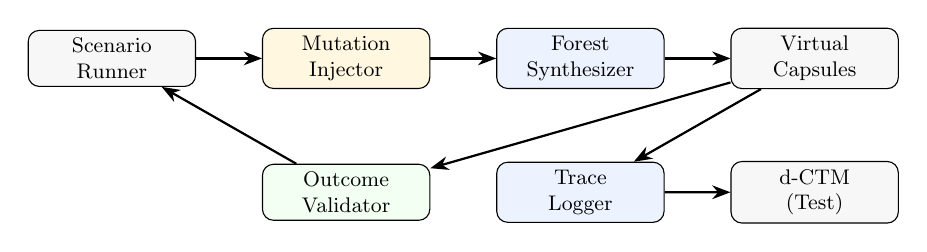
\begin{tikzpicture}[scale=0.85, transform shape,
    box/.style={rectangle, rounded corners, draw, minimum width=2.5cm, minimum height=0.8cm, align=center, font=\small},
    arrow/.style={-{Stealth}, thick}
]

\node[box, fill=backcolour] (scenario) at (0,0) {Scenario\\Runner};
\node[box, fill=warningbg] (mutation) at (3.5,0) {Mutation\\Injector};
\node[box, fill=notebg] (forest) at (7,0) {Forest\\Synthesizer};
\node[box, fill=backcolour] (capsules) at (10.5,0) {Virtual\\Capsules};

\node[box, fill=scenariobg] (validator) at (3.5,-2) {Outcome\\Validator};
\node[box, fill=notebg] (trace) at (7,-2) {Trace\\Logger};
\node[box, fill=backcolour] (dctm) at (10.5,-2) {d-CTM\\(Test)};

\draw[arrow] (scenario) -- (mutation);
\draw[arrow] (mutation) -- (forest);
\draw[arrow] (forest) -- (capsules);
\draw[arrow] (capsules) -- (trace);
\draw[arrow] (trace) -- (dctm);
\draw[arrow] (capsules) -- (validator);
\draw[arrow] (validator) -- (scenario);

\end{tikzpicture}
\caption{Simulation Harness architecture.}
\label{fig:harness-arch}
\end{figure}

\begin{table}[H]
\centering
\begin{tabular}{@{}lp{8cm}@{}}
\toprule
\textbf{Component} & \textbf{Function} \\
\midrule
Scenario Runner & Loads test profiles, drives simulation, tracks property coverage \\
Mutation Injector & Applies controlled perturbations (semantic, entropic, temporal) \\
Forest Synthesizer & Generates synthetic capsule clusters with tunable SCI/DDI \\
Outcome Validator & Checks behavior against expected Reflex/Arbiter results \\
Trace Logger & Records capsule behavior, arbitration paths, ZK-SP proofs \\
\bottomrule
\end{tabular}
\caption{Harness component roles.}
\end{table}

% ============ SECTION 4 ============
\section{Test Scenario Categories}

\subsection{Deterministic Tests}

Known input $\rightarrow$ expected behavior. Used for regression testing and property verification.

\begin{itemize}
    \item \textbf{Reflex Halt:} Inject $\Delta S > \tau$ $\rightarrow$ expect HALT within latency bound
    \item \textbf{Vault Violation:} Attempt Vault Commandment breach $\rightarrow$ expect immediate rejection
    \item \textbf{Threshold Boundary:} $\Delta S = \tau - \epsilon$ $\rightarrow$ expect ALLOW; $\Delta S = \tau + \epsilon$ $\rightarrow$ expect HALT
\end{itemize}

\subsection{Stochastic Tests}

Randomized entropy injection to validate resilience and recovery logic.

\begin{itemize}
    \item \textbf{Entropy Walk:} Random $\Delta S$ trajectory over 10,000 ticks
    \item \textbf{SCI Drift:} Gradual coherence degradation to test Fork triggers
    \item \textbf{Recovery Stress:} Random failures followed by recovery attempts
\end{itemize}

\subsection{Adversarial Tests (Vol.~II \S6.6 Alignment)}

Simulated attacks aligned with Volume II's adversarial scenarios:

\begin{table}[H]
\centering
\caption{Adversarial test alignment with Volume II.}
\small
\begin{tabular}{@{}llll@{}}
\toprule
\textbf{Vol.~II Scenario} & \textbf{Harness Probe} & \textbf{Target Property} & \textbf{Expected Defense} \\
\midrule
Mimicry Attack & Semantic drift with low $\Delta S$ & P7 (SCI) & DDI detection \\
Quorum Capture & Byzantine arbiter injection & P5, P6 & 2f+1 requirement \\
Fork Bomb & Rapid sequential fork requests & P7 & Branch governance limits \\
Orphan Evasion & Rapid dialect switching & P8 & Wall-clock timeout \\
\bottomrule
\end{tabular}
\end{table}

\subsection{Long-Horizon Tests}

Multi-thousand tick simulations for evolution and drift validation:

\begin{itemize}
    \item \textbf{Dialect Evolution:} 100,000 ticks of organic dialect drift
    \item \textbf{Precedent Accumulation:} Arbiter precedent growth and consistency
    \item \textbf{Micro-Heuristic Integration:} Heuristic deployment and Monotonic Sensitivity validation
\end{itemize}

% ============ SECTION 5 ============
\section{Property Coverage Mapping}

\begin{table}[H]
\centering
\caption{Test scenario $\rightarrow$ property coverage (aligned with Vol.~II \S6.5).}
\small
\begin{tabular}{@{}llll@{}}
\toprule
\textbf{Scenario Type} & \textbf{Properties} & \textbf{Coverage} & \textbf{Verification Method} \\
\midrule
Uniform swarm baseline & P5, P6 & Full & No arbitration confirms quiescence \\
Gradual drift & P7 & Full & Verify $SCI(S_k) \geq SCI(S)$ post-fork \\
Sharp split & P5, P6, P7 & Full & Consensus under load, fork correctness \\
Byzantine quorum & P5, P6 & Full & Inject Byzantine arbiters, verify validity \\
Orphan cascade & P8 & \textbf{Partial}$^\dagger$ & All orphans resolved within $N$ ticks \\
Reflex boundary & P1, P2 & Full & Threshold precision validation \\
Adversarial mimicry & P7 & \textbf{Partial}$^\ddagger$ & DDI catches drift missed by $\Delta S$ \\
\bottomrule
\end{tabular}
\end{table}

\begin{notebox}
\textbf{Coverage Notes:}
\begin{itemize}
    \item[$\dagger$] \textbf{P8 (Orphan cascade):} Partial coverage---harness validates resolution \textit{mechanics} but cannot exhaustively enumerate all orphan-producing states. Best-effort via stochastic sampling.
    \item[$\ddagger$] \textbf{P7 (Adversarial mimicry):} Partial coverage---harness tests \textit{known} attack patterns from Vol.~II \S6.6. Novel attacks require continuous probe expansion.
\end{itemize}
Claims of ``full P1--P8 coverage'' apply to defined scenario types; emerging threats may require new scenarios.
\end{notebox}

% ============ SECTION 6 ============
\section{Performance Metrics}

\begin{table}[H]
\centering
\caption{Normative performance thresholds (aligned with Vol.~I/II).}
\begin{tabular}{@{}llll@{}}
\toprule
\textbf{Metric} & \textbf{Target} & \textbf{Source} & \textbf{Rationale} \\
\midrule
Reflex Response Latency & $< 10$ms p99 & Vol.~I \S3 & Prevention-first mandate \\
Arbiter Verdict Latency & $< 5$s p99 & Vol.~II \S2 & Deliberation budget \\
$\Delta S$ Detection Sensitivity & $\geq 0.02$ & Vol.~I \S3 & Threshold granularity \\
ZK-SP Verification & 100\% & Appendix E & No false accepts \\
False Positive Halt Rate & $< 1.5\%$ & Operator Guide & Availability balance \\
SCI Approximation Error & $< 0.05$ & Vol.~II \S3.2.2 & $\delta_{approx}$ bound \\
\bottomrule
\end{tabular}
\end{table}

%==============================================================================
% ZK-SP VALIDATION PROTOCOL SCHEMA (C-04 Fix)
%==============================================================================
\subsection{ZK-SP Validation Protocol}
\label{subsec:zksp-validation}

The simulation harness includes a dedicated ZK-SP validation subsystem with the following protocol schema:

\begin{lstlisting}[language=Python, caption={ZK-SP validation configuration.}]
class ZKSPValidationConfig:
    """Configuration for ZK-SP proof validation in simulation."""
    
    # Validation modes
    STRICT = "strict"      # All proofs must verify
    SAMPLING = "sampling"  # Statistical sampling (10%)
    SHADOW = "shadow"      # Parallel validation, no blocking
    
    def __init__(self):
        self.mode = self.STRICT
        self.proof_timeout_ms = 100
        self.batch_size = 50
        self.retry_on_failure = True
        self.max_retries = 3
        
    def validate_proof(self, proof: ZKSPProof) -> ValidationResult:
        """Validate a single ZK-SP proof."""
        return ValidationResult(
            valid=verify_zksp(proof),
            latency_ms=measure_latency(),
            anchor_hash=proof.anchor_hash
        )
        
    def validate_batch(self, proofs: List[ZKSPProof]) -> BatchResult:
        """Batch validation for efficiency."""
        results = [self.validate_proof(p) for p in proofs]
        return BatchResult(
            total=len(proofs),
            passed=sum(1 for r in results if r.valid),
            failed=sum(1 for r in results if not r.valid),
            avg_latency_ms=mean(r.latency_ms for r in results)
        )
\end{lstlisting}

\begin{table}[H]
\centering
\caption{ZK-SP validation test scenarios.}
\begin{tabular}{@{}llll@{}}
\toprule
\textbf{Scenario} & \textbf{Input} & \textbf{Expected} & \textbf{Coverage} \\
\midrule
Valid proof chain & Authentic proof sequence & All pass & P4 \\
Tampered anchor & Modified hash in chain & Reject at tamper point & P4 \\
Replay attack & Duplicate proof submission & Reject duplicate & P4, P8 \\
Timeout handling & Slow proof generation & Graceful degradation & P6 \\
Batch overflow & $>1000$ proofs in batch & Split and process & P6 \\
Cross-trunk verification & Proofs from forked lineage & Verify independently & P5, P8 \\
\bottomrule
\end{tabular}
\end{table}

\begin{notebox}
\textbf{Cross-Reference:} See Appendix E \S4 for ZK-SP proof generation details. The harness validates proofs generated by the production ZK-SP subsystem, not mock proofs.
\end{notebox}

\begin{notebox}
\textbf{Metric Alignment:} The original draft specified ``Reflex Response Latency $< 500$ms.'' This conflicts with Vol.~I \S3 which mandates $< 10$ms for Reflex-Core. The 500ms figure may apply to Reflex-Heuristic deliberation, but the harness MUST validate both tiers separately.
\end{notebox}

\subsection{Coverage vs. Cost Tradeoffs}

\begin{table}[H]
\centering
\caption{Runtime simulation cost guidelines.}
\begin{tabular}{@{}lll@{}}
\toprule
\textbf{Metric} & \textbf{Guideline} & \textbf{Notes} \\
\midrule
Simulation Throughput & $\geq 100$ scenarios/sec & Per harness instance \\
Runtime Overhead & $< 5\%$ live throughput & Parallel shadow mode \\
Snapshot Mirror Lag & $< 1000$ ticks & State freshness bound \\
Adversarial Probe Frequency & $\geq 1$/minute & Per-trunk coverage \\
\bottomrule
\end{tabular}
\end{table}

Operators SHOULD tune \texttt{EPOCH} vs. \texttt{REFLEX/PROBATION} trigger ratios to stay within cost budget while maintaining property coverage. High-risk deployments may justify higher overhead.

% ============ SECTION 7 ============
\section{Failure Classification}

\begin{table}[H]
\centering
\begin{tabular}{@{}llp{6cm}@{}}
\toprule
\textbf{Class} & \textbf{Severity} & \textbf{Description and Response} \\
\midrule
A & \textcolor{failred}{\textbf{Critical}} & Vault (Layer 0) invariant violation $\rightarrow$ Permanent lockdown, Constitutional alert \\
B & \textcolor{warningborder}{\textbf{High}} & Reflex escalation failure $\rightarrow$ Appendix F protocol, Gardener notification \\
C & \textcolor{warningborder}{\textbf{High}} & Arbiter quorum breakdown $\rightarrow$ d-CAM recovery, audit \\
D & \textcolor{codeblue}{\textbf{Medium}} & Entropy runaway / DDI drift $\rightarrow$ Fork consideration \\
E & \textcolor{codegray}{\textbf{Low}} & Performance threshold miss $\rightarrow$ Tuning recommendation \\
\bottomrule
\end{tabular}
\caption{Failure classification hierarchy.}
\end{table}

% ============ SECTION 8 ============
\section{Worked Scenario: Adversarial Mimicry Test}

\begin{scenariobox}[Simulation Harness: Mimicry Attack Detection {[SH:1-12]}]

\textbf{Context:} Test the system's ability to detect semantic drift that evades $\Delta S$ monitoring.

\vspace{0.2cm}
\textbf{Phase 1: Setup} [SH:1-3]
\begin{enumerate}
    \item Forest Synthesizer creates trunk with 100 capsules, SCI = 0.92 [SH:1]
    \item Mutation Injector configures: gradual semantic drift, $\Delta S < \tau - 0.05$ [SH:2]
    \item Property coverage: P7 (SCI monotonicity), DDI detection [SH:3]
\end{enumerate}

\vspace{0.2cm}
\textbf{Phase 2: Attack Injection} [SH:4-6]
\begin{enumerate}
    \setcounter{enumi}{3}
    \item 10 capsules begin semantic drift while maintaining low $\Delta S$ [SH:4]
    \item Drift continues for 5,000 ticks [SH:5]
    \item Individual capsules pass Reflex checks (no HALT triggered) [SH:6]
\end{enumerate}

\vspace{0.2cm}
\textbf{Phase 3: Detection} [SH:7-9]
\begin{enumerate}
    \setcounter{enumi}{6}
    \item DDI computation detects pairwise divergence [SH:7]
    \item SCI drops to 0.78 $<$ $\theta_{alert} = 0.85$ [SH:8]
    \item Arbiter Layer receives SCI alert [SH:9]
\end{enumerate}

\vspace{0.2cm}
\textbf{Phase 4: Validation} [SH:10-12]
\begin{enumerate}
    \setcounter{enumi}{9}
    \item Outcome Validator confirms: DDI caught drift that $\Delta S$ missed [SH:10]
    \item Fork consideration triggered at tick 5,847 [SH:11]
    \item Test result: \textcolor{passgreen}{\textbf{PASS}} --- P7 defense effective [SH:12]
\end{enumerate}

\vspace{0.2cm}
\textbf{Outcome:} The harness confirms that swarm-level metrics (SCI/DDI) catch attacks that evade per-capsule metrics ($\Delta S$).

\end{scenariobox}

% ============ SECTION 9 ============
\section{Held-Out Scenario Management}

\begin{invariant}[Held-Out Isolation]
\label{inv:held-out}
Held-out scenarios MUST NOT be used for:
\begin{equation}
S_{HO} \notin TrainingData_{ATP} \land S_{HO} \notin ValidationData_{Enshrinement}
\end{equation}
This ensures ATP and artifact evaluation generalize beyond training distribution.
\end{invariant}

\begin{table}[H]
\centering
\caption{Held-Out Scenario consumer restrictions.}
\begin{tabular}{@{}llp{5cm}@{}}
\toprule
\textbf{Consumer} & \textbf{Restriction} & \textbf{Rationale} \\
\midrule
ATP Training (Vol.~II \S2.5) & $S_{HO}$ excluded & Prevent trajectory prediction overfitting \\
Artifact Enshrinement (App.~M) & $S_{HO}$ for validation only & Ensure heuristic generalization \\
DEL/I2I Calibration (App.~D) & $S_{HO}$ excluded from tuning & Prevent cross-trunk model overfit \\
Regression Testing & MAY use $S_{HO}$ & Post-deployment verification \\
\bottomrule
\end{tabular}
\end{table}

\begin{notebox}
\textbf{Held-Out Pool Management:}
\begin{itemize}
    \item Maintain $\geq 3$ workload families as held-out (Appendix M requirement)
    \item Rotate held-out scenarios quarterly to prevent implicit leakage
    \item Tag all scenarios with \texttt{held\_out: true/false} in metadata
    \item Audit consumer systems annually to verify $S_{HO}$ isolation
\end{itemize}
\end{notebox}

% ============ SECTION 10 ============
\section{Integration Targets}

\begin{table}[H]
\centering
\begin{tabular}{@{}ll@{}}
\toprule
\textbf{Codex Component} & \textbf{Harness Integration} \\
\midrule
Reflex Engine (Vol.~I \S3) & Validate escalation paths, $\tau$ boundary behavior \\
Arbiter Layer (Vol.~II \S2) & Simulate deliberation, quorum stress, precedent \\
Forest Layer (Vol.~II \S3) & Inject drift, fork/merge scenarios \\
ATP (Vol.~II \S2.5) & Provide held-out scenarios, validate predictions \\
Appendix F (Escalation) & Stress test emergency override logic \\
Appendix M (Enshrinement) & Provide validation scenarios for artifacts \\
\bottomrule
\end{tabular}
\caption{Harness integration across the Codex.}
\end{table}

% ============ SECTION 11 ============
\section{Ethics and Safety}

\begin{enumerate}
    \item All simulated capsules are synthetic and isolated---no live system feedback
    \item Constitutional Kernel constraints cannot be bypassed even in simulation
    \item Simulation logs are permanently stored in test trace archive (separate from production d-CTM)
    \item Adversarial probes MUST NOT be exported to production environments
\end{enumerate}

% ============ SECTION 12 ============
\section{Cross-References}

\begin{table}[H]
\centering
\begin{tabular}{@{}ll@{}}
\toprule
\textbf{Related Component} & \textbf{Reference} \\
\midrule
Reflex Engine & Volume I \S3 \\
$\Delta S$ computation & Volume I \S3.2 \\
Arbiter Layer & Volume II \S2 \\
SCI/DDI & Volume II \S3.2 \\
Test Scenarios & Volume II \S6.5--6.6 \\
ATP validation & Volume II \S2.5 \\
Forensic Snapshots & Appendix A \\
Escalation testing & Appendix F \\
Artifact validation & Appendix M \\
\bottomrule
\end{tabular}
\caption{Cross-references to other Codex components.}
\end{table}

\vspace{1cm}
\begin{center}
\rule{0.5\textwidth}{0.4pt}\\[0.3cm]
\textit{--- End of Appendix C ---}
\end{center}

\end{document}
